    \documentclass[12pt,letterpaper]{article}

\usepackage[utf8]{inputenc}
\usepackage{natbib}
\usepackage{graphicx}
\usepackage{indentfirst}
\usepackage{amsmath}
\usepackage{amsfonts}
\usepackage{amssymb}
\usepackage{comment}
\usepackage{url}
\usepackage[left=3cm,right=2cm,top=2cm,bottom=3cm]{geometry}
\usepackage{titlesec}

\setlength{\parindent}{2cm}
\renewcommand{\baselinestretch}{1.5}
\renewcommand\contentsname{Tabla de contenidos}
\renewcommand\refname{Referencias}
\renewcommand\figurename{Figura}

\begin{document}

\newpage
\vspace*{-.5cm}
\begin{picture}(18,4)(0,30)
	\put(350,-20){
\includegraphics[scale=0.25]{./images/LogoUsach.pdf}}
\end{picture}

\sloppy
\thispagestyle{empty}
\vspace*{-1.6cm}

\begin{center}
	{\bf \mbox{\large UNIVERSIDAD DE SANTIAGO DE CHILE}}\\
	{\bf \mbox{FACULTAD DE INGENIER\'IA}}\\
	{\bf \mbox{DEPARTAMENTO DE INGENIER\'IA INFORM\'ATICA}}\\
\end{center}

	\vspace*{3cm}
	\par
	\vspace{1cm}
	\begin{center}
	\large
		%Algoritmos de predicci\'on y distribuci\'on de carga para motores de procesamiento de \textsl{stream}
		Algoritmos de predicci\'on y distribuci\'on de carga para el grafo lógico en los motores de procesamiento de \textsl{stream}
	\end{center}

	\vspace{0.5cm}
	\begin{center}
	\large
		\textbf{Propuesta de tesis}
	\end{center}
	
	\vspace*{4.25cm}
	\begin{flushright}
		\begin{tabular}[t]{l l}
			Nombre: & Daniel Pedro Pablo Wladdimiro Cottet \\
			R.U.N.: & 18.294.093-3\\
			Carrera: & Magíster en Ingeniería Informática\\
			A\~no estimado de egreso: & 2015\\
			Tel\'efono: & +56 9 82966028\\
			E-mail: & daniel.wladdimiro@usach.cl\\
			Profesor guía: & Nicolás Hidalgo Castillo\\
			Profesora co-guía: & Erika Rosas Olivos

		\end{tabular}
	\end{flushright}
	\begin{center}
		\vspace{1.5cm}
		Jueves, 4 de diciembre de 2014
	\end{center}

\newpage
\tableofcontents
\thispagestyle{empty}

\newpage
\renewcommand{\thepage}{\arabic{page}}
\setcounter{page}{1}

\section{Descripción del problema}
\subsection{Motivación}
% RANNOU: Describe el contexto donde surge el problema, la situación actual. Argumenta sobre la importancia que tiene cambiar esta situación por una deseada el impacto esperado o las consecuencias más relevantes, que una solución tendría en las personas, en las empresas o en alguna disciplina de conocimiento. Los argumentos aquí presentados, en relación con la importancia del desarrollo de una solución, son antecedentes necesarios para justificar la realización de la tesis.

%Cloud; a posteriori 

La gran contribución de información en la Internet se ha debido al origen de la Web 2.0,
donde ésta se caracteriza por la participación activa del usuario, siendo reflejado en el auge de blogs, redes sociales u otras aplicaciones web \cite{web2007oberhelman}. Debido a lo anterior, se crean sistemas de procesamiento para grandes cantidades de información generadas por la interacción entre los usuarios.

Es así como con el tiempo se han ido creando distintas aplicaciones de \textsl{streaming}, debido al interesante funcionamiento que poseen, las que se caracterizan por ser capaces de procesar grandes flujos de datos en tiempo real \cite{ChenZ14a}. La necesidad de procesar informaci\'on en tiempo real surge dado que muchas aplicaciones, donde sus usuarios requieren de respuestas r\'apidas y actualizadas que le permitan tomar decisiones en per\'iodos cortos de tiempo. Dentro de los ejemplos existentes se encuentran; análisis de sentimientos de los mensajes de usuarios, análisis de los precios de la bolsa de valores, recopilación de información en caso de emergencia, entre otros. Las distintas aplicaciones que se han creado se volvieron críticas para sus usuarios, debido que sustenta la toma de decisiones de empresas o instituciones \cite{Wenzel14}.

%Rannou dice que es muy breve, chamullar más...
Entre los sistemas actuales de procesamiento de \textsl{streaming} se encuentran S4 \cite{s4yahoo}, Storm \cite{stormtwitter}, Samza \cite{samza}, entre otros, los cuales son los más utilizados como arquitectura de procesamiento en la confección de distintas aplicaciones de \textsl{streaming}. Aunque poseen bastante flexibilidad para la creación de un sistema, por la facilidad de crear distintas topologías, no lo tiene para adaptarse en el tiempo, debido a que las topolog\'ias de procesamiento generadas son est\'aticas, por lo que dada la naturaleza din\'amica de las interacciones pueden surgir problemas de sobrecarga.

%El problema de sobrecarga conlleva a una baja en el rendimiento, produciendo una pérdida de recursos, tiempo o información. Al encontrar una solución a esto, se tiene una mejora en la exactitud y disminución en el tiempo de procesamiento, debido que al tener mayor cantidad de datos, dado el menor tiempo de procesamiento de éstos, se obtiene una mayor exactitud en la información entregada. De esta manera, se efectúa una optimización en los recursos utilizados, una mejora en el tiempo de procesamiento y mayor la calidad de la información entregada.

El problema de sobrecarga conlleva a una baja en el rendimiento, produciendo una pérdida de recursos, tiempo o información. Abortar este problema es cr\'itico, puesto que implica una mejora en la exactitud y disminución en el tiempo de procesamiento, debido que al tener mayor cantidad de datos, menor tiempo de procesamiento, se mejora la información entregada. Un ejemplo de esto, es que se posee un tiempo $t$ para procesar $n$ datos, de disminuir el tiempo de procesamiento total de los datos, se tendrá que en el mismo tiempo $t$ se procesarán una cantidad $n+m$ de datos, donde $m$ son los datos adicionales a analizar debido a la mejora del rendimiento. Como existe una mejora en la cantidad de datos para analizar, la información de salida es más exacta, debido que tiene más datos con que comparar. De esta manera, se efectúa una mejora en los recursos utilizados, debido a la disminución del tiempo de procesamiento, y una mejor calidad en la información entregada al usuario.

\subsection{Dominio del problema}
% RANNOU: Presenta sucintamente los principales conceptos del dominio del problema y las relaciones entre ellos, necesarios para entender con mayor profundidad el problema que se describe en esta propuesta.


Entre los diferentes motores de procesamiento de datos masivos, existen los motores de \textsl{streaming}, los cuales reciben grandes cantidades de datos que deben procesar de forma distribuida y \textsl{online}. Para realizar esto, se requiere un cambio en el paradigma \textsl{bash processing}, el cual guarda los datos en una base de datos, los cuales luego son procesados de forma \textsl{offline} \cite{HawwashN14}, a uno que procese de forma \textsl{online}. Por lo que el paradigma cambia a uno basado en grafos, donde a través del cual fluye un \textsl{stream} de datos que es procesamiento por el conjunto de operadores que lo componen, los operadores corresponden a los nodos del grafo y las aristas a los flujos de datos preprocesados que salen del operador \cite{Shahrivari14}.

El modelo de procesamiento que se muestra en la Figura \ref{fig:grafo}, corresponde a un SPE (Sistema de Procesamiento de Eventos). Los vértices corresponden a operadores, como por ejemplo analizadores de sentimientos, filtros de palabras o algún algoritmo en particular, y las aristas corresponden a los flujos de datos entre un operador y otro. Además de esto, se tiene una fuente de datos, la cual entrega los datos iniciales a los primeros operadores del grafo \cite{AppelFFB12}.

\begin{figure}[ht!]
  \centering
    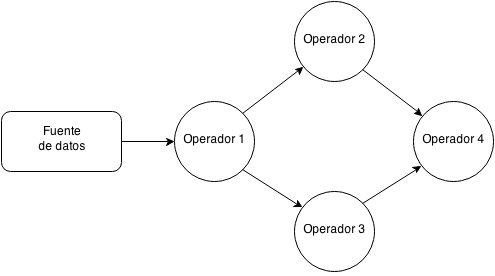
\includegraphics[scale=0.5]{images/Grafo.png}
  \caption{Ejemplo de modelo de SPE.}
  \label{fig:grafo}
\end{figure}

Cada motor de procesamiento de \textsl{streaming} está basado en un modelo de procesamiento en particular. Por ejemplo, S4 está basado en el modelo de procesamiento \textsl{push} \cite{s4yahoo}, y Storm en el modelo \textsl{pull} \cite{stormtwitter}. El primer modelo consiste en el envío de datos desde el operador. La ventaja de este modelo empleado por S4 radica en la abstracción en el envío de datos, sin embargo no asegura el procesamiento de estos, debido a que no existe un mensaje de respuesta al ser entregado al operador. En cambio, en el segundo modelo se basa en la petición de datos a un operador, por lo que son enviados solo si son requeridos. Si bien este modelo asegura procesamiento de los datos, genera una menor abstracción al programador, dado que en el primer modelo sólo se programa a que operador debe ir, en cambio en el segundo se debe indicar quién lo envía y quién lo recibe.

Pues bien, independiente del método que se utilice, existe un problema en la distribución, dado el dinamismo de los datos a procesar, pudiendo generarse sobrecargas en algún operador. Esto se produce dado que la tasa de procesamiento es menor a la tasa de llegada, generando colas en el sistema \cite{queueingtheory}. Por ejemplo, si se posee una tasa de llegada $\lambda$ y una tasa de servicio $\mu$, donde $\mu < \lambda$, se generan colas en el sistema, debido que se procesa más lento de lo que llegan los datos. Como existen colas, es necesario un aumento del rendimiento del sistema, debido que $\rho > 1 $, donde se define $\rho = \frac{\lambda}{s\mu}$, siendo $s$ la cantidad de servicios disponibles.

El caso más simple de modelo de SPE, existe una réplica por cada operador, de esta manera, cada servicio tendrá un valor de 1. Por lo tanto, al crear réplicas de cada uno de los servicios, se aumenta el rendimiento del sistema, en caso de haber colas. Para no utilizar recursos de forma excesiva, es necesario realizar el proceso de forma elástica, la cual se define como el aumento o disminución de la cantidad de servicios según la cantidad requerida por el sistema.

%Por lo tanto, es importante dar solución a las sobrecargas en los operadores, de tal manera que haya una menor tiempo promedio de espera en el procesamiento de los datos. Además, se tiene una mayor exactitud en los datos entregados, debido que la información entregada es más pŕoxima al tiempo real.

Es importante dar una solución al problema de sobrecarga de los operadores, para disminuir el tiempo del  procesamiento y aumentar la precisión de los resultados del sistema.

\subsection{Definición del problema}
Dada la falta de flexibilidad del modelo de procesamiento de \textsl{streams}, surge un problema basado en la sobrecargada de los operadores más demandados. Esto debido a que no existe una forma de disminuir la sobrecarga y reducir las colas de espera, para mejorar el rendimiento del sistema y obtener información cercana al tiempo real.

\section{Objetivos del proyecto}
\subsection{Objetivo general del proyecto}
Dise\~no, construcción y evaluaci\'on de un algoritmo de predicci\'on y un algoritmo de distribuci\'on de carga para motores de procesamiento de \textsl{stream}.

\subsection{Objetivos específicos}
\begin{itemize}
%\item Dise\~nar e implementar un algoritmo de monitoreo que permita medir la carga de los operadores.
%\item Dise\~nar e implementar un algoritmo h\'ibrido que permita analizar y estimar la carga de los operadores.
\item Dise\~nar e implementar un algoritmo de predicci\'on que permita estimar la carga de los operadores.
\item Dise\~nar e implementar un algoritmo de distribuci\'on que permita la administraci\'on de los operadores del grafo de procesamiento de forma el\'astica.
\item Dise\~nar y construir experimentos que permitan validar la hip\'otesis formulada.
%\item Dise\~nar e implementar un algoritmo para administrar los operadores de forma elástica en el grafo de procesamiento.
\item Evaluar y analizar el rendimiento del sistema a trav\'es de aplicaciones generadas sobre procesamiento de motores de \textsl{stream}.
\end{itemize}

\section{Descripción de la solución propuesta}
\subsection{Estado del arte}
%Rannou: Estado del arte de un objetivo de estudio se refiere al estado mas elevado de desarrollo alcanzado por el objeto en un momento particular. En este caso el objeto de estudio es la solución del problema que puede ser un producto de un software, un método, un modelo una teoría etc. En esta sección se espera una revisión de los fundamentos teóricos del objeto de estudio, los antecedentes que hay del tema expresado en dos formas primero una breve descripción de su evolución y luego una descripción resumida del estado del arte actual (últimos años), desde dos perspectivas: nacional e internacional.

Dentro de la literatura se han encontrado distintas perspectivas al problema de balance de carga en un SPS (Sistema de Procesamiento de \textsl{Streaming}). Una perspectiva es respecto a los recursos físicos, donde se define la sobrecarga de un nodo por la cantidad de operadores que posee \cite{MadsenTZ14}. Una solución es lo realizado por Borealis; éste realiza un balanceador según la carga de los nodos \cite{XingZH05}, de tal manera de enviar las tareas a los nodos menos sobrecargados. Otra perspectiva es a nivel lógico, la cual está orientada en el grafo de operadores, donde el problema está en la sobrecarga de un operador \cite{FernandezMKP13}. Este problema se debe a que un operador puede sobrecargarse, formando cuellos de botella y  esperas en el sistema. Una de las soluciones, es lo presentando por Schneider que corresponde a la paralelización de una tarea que posea distintos operadores \cite{SchneiderAGBW09}, de tal manera que cada tarea pueda trabajar de forma independiente y no sobrecargar un nodo. Otra solución es lo presentando por Fernández \cite{FernandezMKP13}, el cual consiste en la replicación de un operador según la sobrecarga de algún operador en el grafo, de tal manera de detectarlo y crear una réplica de éste para que puedan ambos operadores trabajar en conjunto para la operación demandada.

Por lo tanto, para realizar optimizaciones al sistema se han presentando dos tipos de enfoques: el estático y el dinámico \cite{Dong06schedulingalgorithms}. El primer enfoque se centra en la confección de un modelo definido y fijo antes de iniciar el sistema y que no varía en el tiempo. En cambio, el segundo se basa en la adaptación del sistema según su estado en tiempo de ejecución.

\addtocontents{toc}{\protect\setcounter{tocdepth}{1}}
\subsubsection{Enfoque estático}

Este enfoque se ha implementando en distintos motores de \textsl{streaming}, donde no se depende del estado del sistema \cite{stormtwitter, s4}. De esta manera, no existe una interrupción en la ejecución o un cambio en las variables  \cite{CasavantK88}. Esto significa, que al momento de distribuir los distintos operadores, esto se realiza homogéneamente, independiente de la carga, latencia u otro estado del sistema.

\textsl{Storm} utiliza la técnica de distribución de operadores según alguna política, tomando el enfoque estático \cite{stormtwitter}. El sistema configura el número de operadores que son necesarios para realizar una tarea, para que después estos sean repartidos en los distintos nodos disponibles según la política de \textit{Shuffle grouping}. Esta técnica basada en algoritmos de planificación \cite{bookScheduling}, consiste en distribuir los operadores en los distintos nodos utilizando una planificación \textsl{Round-Robin}, de tal manera que la cantidad de operadores sea uniforme en los nodos del sistema \cite{bookstorm}.

Otra técnica es el uso de la función \textsl{hash} \cite{RogawayS04} para distribuir los operadores en el grafo, como lo planteado en S4 \cite{s4yahoo}. Esto consiste en aplicar lo anterior a algún atributo del evento, mapeando el evento al operador que corresponda de los $n$ operadores disponibles según el valor de la función. Cabe destacar que si no existe un operador mapeado con la imagen de la función, el sistema clona uno existente evaluando el nuevo con la imagen de la función como identificador. De esta manera, esta técnica provee dinamicidad respecto a la cantidad de operadores en el sistema.

Una ventaja del enfoque estático es el bajo costo de la implementación de los métodos, lo cual es beneficioso para sistemas con bajos recursos. Por otra parte, una desventaja existente es la sobrecarga de un nodo u operador, debido que no asegura que alguno de ellos tenga una mayor tasa de procesamiento que la tasa de llegada. Si bien, no es una solución óptima, es un buen complemento para un modelo con el enfoque dinámico.

\addtocontents{toc}{\protect\setcounter{tocdepth}{2}}
\subsubsection{Enfoque dinámico}

Este enfoque está basado en el estado del sistema, donde según las variables y estado de cada uno de sus atributos, genera una acción en el sistema \cite{CasavantK88}. Esto significa que si el sistema posee alguna anomalía, como una sobrecarga en un operador o latencia entre distintos nodos, se realiza un cambio en el sistema, con el fin de solucionar estos problemas. Para poder dar una solución al problema de sobrecarga, se pueden utilizar dos tipos de modelos: reactivo y predictivo.

\paragraph{Reactivo}

Este modelo está basado en la detección de sobrecargas en el sistema a través de un monitor \cite{GulisanoJPSV12}. El monitor recibe periódicamente la carga de cada uno de los nodos u operadores, y en caso que se sobrepase un umbral, se aplica una técnica para aumentar el rendimiento bajo una métrica dada. El umbral puede estar basado en el tiempo de procesamiento, el tamaño de la cola u otra variable del nodo u operador \cite{BhuvanagiriGKS06}. Por ejemplo, para realizar una paralelización de un operador sobrecargado, se utiliza un algoritmo que analiza si los operadores sobrepasan un umbral propuesta, el cual está determinado por la frecuencia máxima de llegada de ellos según el tasa de procesamiento del operador \cite{SchneiderAGBW09}.

\paragraph{Predictivo}
El modelo predictivo está basado en modelos matemáticos que puedan simular la actividad del operador, y predecir la carga de éste. Primero se determina la carga de un operador en cierto período de tiempo, y después se aplica un modelo matemático que predice la carga en el próximo intervalo de tiempo. La predicción de carga de cada operador se realiza mediante modelos de Markov \cite{GongGW10}, y analizando si existe alguna sobrecarga en los operadores a futuro. Si bien lo anterior no ha sido implementando en el contexto de \textsl{Stream}, si se ha realizado en \textsl{Cloud Computing} según la sobrecarga de los computadores \cite{NguyenSGSW13}.\\

Existen distintas técnicas que son utilizadas en ambos modelos, entre las cuales están la planificación determinista \cite{XuCTS14, DongTS07}, descarte de eventos \cite{SheuC09}, migración \cite{XingZH05}, para\-lelización \cite{GulisanoJPSV12, IshiiS11, GedikSHW14} y replicación \cite{FernandezMKP13}.

La planificación determinista \cite{DongTS07} se centra en la planificación según los recursos y estados del sistema \textsl{a priori} según alguna métrica \cite{XuCTS14}. Una métrica utilizada es la frecuencia de datos estimada en un nodo u operador \cite{Ganguly09}. Esta técnica se utiliza, por ejemplo, en \textsl{StreamIt} \cite{ThiesKA02}. Una de las limitaciones es que si bien realiza una predicción determinista de la frecuencia, no necesariamente es correcta a futuro, por lo que no se puede predecir las tasas de tráfico en el transcurso del procesamiento, sino sólo estimarlas al comienzo de la ejecución del sistema.

Otra estrategia está orientada a descartar eventos de un operador sobrecargado, de tal manera de no generar colas en el sistema. Esta estrategia que si bien no está implementada en el sistema por defecto de S4, puede habilitarse \cite{s4}. Otro ejemplo, es la trasmisión de vídeo \textsl{streaming}, donde se descartan los datos que son de baja calidad, para procesar en su mayoría información de alta calidad \cite{SheuC09}. Esta solución está pensada para disminuir la carga, perdiendo la exactitud de la información debido a la pérdida de datos. Por lo tanto existe una menor fiabilidad en el sistema en caso de realizar operaciones de transacción \cite{bookDistrSys}.

También se encuentra la migración, en el cual según el estado del sistema se migran los operadores de un nodo a otro. En \cite{XingZH05} se implementa   esta técnica, y si bien genera una menor carga en distintos nodos, produce un alto costo en la transferencia de los datos. Al realizar la transferencia de los datos, existe una menor tolerancia a fallos, a raíz de lo cual, se propone el uso de un búffer en el sistema, aumentando sus costos \cite{PittauACA07}.

Desde otra perspectiva, existen las técnicas de paralelización y replicación, las cuales se utilizan en caso de sobrepasar un umbral, el cual depende de la carga de un operador, nodo, entre otras variables. El primero consiste en paralelizar una tarea, la cual está determinada por un conjunto de operadores, en otro nodo físico \cite{IshiiS11}. En cambio, la replicación consiste en replicar un operador a nivel lógico del grafo \cite{MadsenTZ14}. Una de las características que existen en este tipo de soluciones es la elasticidad, que consiste en la capacidad de aumentar o disminuir la cantidad de operadores según la necesidad del sistema.

Una aplicación de la técnica de paralelización según el enfoque estático, es la paralelización de tareas de Storm \cite{stormtwitterdoc}, donde un conjunto de operadores realizan una tarea, indicado la cantidad de tareas que se desean ejecutar paralelamente en el sistema. Un ejemplo aplicado de esta técnica según el enfoque dińamico es StreamCloud \cite{GulisanoJPSV12}, que dada la cantidad de consultas que van llegando al sistema, se paralelizan las tareas existentes. Uno de los problemas que surge en estos casos son las operaciones con estado, como lo son los contadores o algoritmos de orden. La solución planteada es poseer un operador que realiza la tarea de \textsl{merge}, que consiste en recibir las salidas de las tareas paralelas, agrupando los datos y proporcionando una salida según lo realizado por cada uno de las operaciones \cite{GedikSHW14}.

Por otra parte, se usa la técnica de replicación en una aplicación diseñada por Fernández \cite{FernandezMKP13}. Ésta está enfocada en la replicación de operadores, la cual se activa si se detecta un cuello botella en el procesamiento de los datos. Para la detección, existe un monitor que está recibiendo la carga de cada uno de los procesos, y si es sobrepasado el umbral, debe realizar una petición de replicación al operador sobrecargado.

\subsection{Características de la solución}
% RANNOU: Se propone una solución en función del problema planteado. Se indican las principales características o requisitos que debe cumplir la solución, Se describe la solución desde la perspectiva de la ingeniería informática. La solución debe tener correspondencia con el objetivo general del proyecto, por ejemplo, puede ser el desarrollo de un sistema de software o evaluación o comparación de aplicaciones o métodos desarrollo y/o evaluación de modelos o de una teoría.

La solución propuesta consiste en el dise\~no de algoritmos de predicci\'on y distribuci\'on de carga a nivel de la l\'ogica del grafo. En la Figura \ref{fig:opt} se muestran los cuatro módulos que componen la estructura del m\'odelo propuesto para el dise\~no de los algoritmos, los cuales se componen por el monitor de carga, analizador de carga, predictor de carga y administrador de réplicas.

\begin{figure}[ht!]
  \centering
    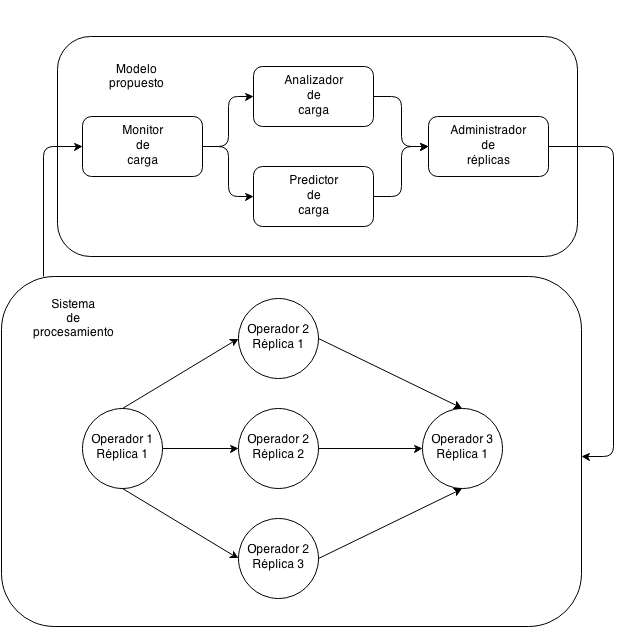
\includegraphics[scale=0.5]{images/Diagrama.png}
  \caption{Estructura del sistema de operadores y modelo propuesto.}
  \label{fig:opt}
\end{figure}

El monitor de carga está encargado de recuperar el nivel de carga de cada uno de los operadores. Esta información es entregada a otros dos módulos, los cuales están encargados de procesarla de tal manera de ver si existe alguna sobrecarga. Cada uno de éstos trabaja de forma independiente y tiene distintos métodos, uno proactivo y otro reactivo, de tal manera de poseer mayor exactitud en la detección de una sobrecarga.

El analizador de carga consiste en un método reactivo, el cual analiza el tráfico de los operadores en el tiempo actual, y cuantifica su carga. La sobrecarga de cada operador depende de un umbral, por lo que según ésto se envía al administrador de réplica el tráfico de cierto operador de ser necesario una replicación.

El predictor de carga consiste en un método proactivo, el cual analiza la carga de los distintos operadores según una ventana de tiempo, y predice la carga según un método predictivo. De esta manera, se determina la posible carga que existe en cierto período de tiempo futuro, donde según un umbral y un margen de error se envía el tráfico de carga de un operador al administrador de réplicas, y así analizar si es necesario una replicación.

El administrador de réplicas se alimenta de la información entregada por los dos módulos anteriores, y así toma una decisión de la administración de cada una de las réplicas de los distintos operadores. Por lo tanto, verifica cuántas réplicas son necesarias según la cantidad de tráfico de cierto operador.

Finalmente, el sistema de procesamiento constantemente está realizando un \textsl{feedback} al sistema de optimización, de tal manera que pueda administrar las réplicas necesarias.

%HIPOTESIS
Este sistema dar\'a un procesamiento más rápido de la información entregada en el sistema de procesamiento \textsl{online} de datos, a través de un proceso de optimización que posea bajo \textsl{overhead}.

\subsection{Propósito de la solución}
% RANNOU: Se indica el propósito de los resultados de las tesis. Corresponde al objetivo final que tiene en mente el cliente o el beneficio que se espera reciba el destinatario de la solución. Indica en qué medidas mejoraría la situación actual del problema.

Dada la formación de colas y retraso en la salida de los datos en los operadores, se plantea un sistema de optimización para los motores de \textsl{streaming} que trabajen con módulos proactivos y reactivos. Esto será un beneficio para el procesamiento de los datos en tiempo \textsl{online}, de tal manera de obtener información de forma más rápida y con mayor exactitud.

\subsection{Alcance o limitaciones de la solución}
% RANNOU: Se deja establecido con claridad qué debe considerarse como parte del trabajo y que no, y el grado de satisfacción esperado, Junto con el punto anterior, este punto permite saber si el estudiante no hará menos de lo que se quiere, o más de lo que se debe.

Dentro de los alcances y limitaciones que se tienen en el proyecto son:
\begin{itemize}
\item La evaluación de la solución presentada se implementará sobre un solo motor de procesamiento de \textsl{streaming} a definir.
%\item Se experimentará con diferentes aplicaciones con restricciones de tiempo de respuesta y con dinamismo en su flujo de datos.
\item Se evaluará con al menos dos aplicaciones bajo escenarios simulados utilizando datos reales.
\item La distribución de flujo de datos será a nivel de operadores y no de nodos f\'isicos, por lo que no se analizará la carga de estos \'ultimos.
%\item No se realizará un algoritmo o un sistema que pueda detectar falsas alarmas de sobrecarga, de tal manera que puedan cancelar las réplicas que se deseen crear.
%\item Se utilizarán algoritmos reactivos y predictivos del estado del arte en la implementación para comparar resultados.
\item Los algoritmos propuestos no incluyen t\'ecnicas que garanticen el procesamiento de todo el flujo de datos.
\item En la evaluación de los algoritmos propuestos se considerará el costo de comunicación de manera igualitaria para todos los operadores.
\item Se comparará la solución con dos motores de procesamiento de \textsl{stream} del estado del arte.
\end{itemize}

\section{Metodología, herramientas y ambiente de desarrollo}
\subsection{Metodología a usar}
Dado el carácter de investigación de la propuesta de tesis, se propone utilizar el método científico para la realización de ésta. Dentro de las etapas propuesta por \cite{hernandez2010metodologia} están:

\begin{enumerate}
\item Formulación de la hipótesis: ``La utilización de un modelo híbrido de paralelización permitirá mejorar la distribución de carga entre los operadores de manera dinámica logrando reducir los tiempos de procesamiento y pérdida de eventos".
%\item Formulación de la hipótesis: "Es posible dise\~nar algoritmos de predicci\'on y distribuci\'on de carga para SPE, que resuelva el problema de sobrecarga en los operadores del sistema, aumentando así su rendimiento".
\item Elaboración del marco teórico: Exponer las investigaciones que existen sobre problemas de sobrecarga en los operadores de SPE. Así mismo, los conceptos fundamentales de estos sistemas.
\item Seleccionar el diseño apropiado de investigación: Diseñar el experimento para el problema de balance de carga a nivel lógico en un SPE, vale decir, los algoritmos de predicción y distribución. Cada ejecución de los experimentos se basan según los principios de un SPE.
\item Analizar los resultados: De deberá analizar los resultados según las estadísticas entregadas y el modelo propuesto.
\item Presentar los resultados: Elaborar el reporte de investigación y presentar los resultados en gráficos y tablas.
\item Concluir en base a los resultados de la investigación.
\end{enumerate}

\subsection{Herramientas de desarrollo}
Para el procesamiento de \textsl{stream} se utilizará Apache S4 0.6.0 o Apache Storm 0.9.3, por lo que será necesario para su configuración Java SE Development Kit 8. Dentro esto, el lenguaje de programación de cada una de las estructuras del sistema desarrollado serán en Java, por lo que se trabajará sobre un IDE, el cual será Eclipse Standard 4.3.2, y para el uso de un modelo matemático se utilizará MATLAB 2014a. De forma complementaria, se utilizará Texmaker 4.2 para la confección de los distintos informes requeridos y la documentación correspondiente al trabajo.

\subsection{Ambiente de desarrollo}
El ambiente de desarrollo será llevado a cabo en el computador personal del autor, y para las pruebas en los equipos disponibles de CITIAPS (Centro de Innovación en Tecnologías de la Información para Aplicaciones Sociales) ubicado en la Universidad de Santiago de Chile. Estas herramientas contarán con acceso a Internet y las herramientas necesarias para realizar las pruebas y mediciones correspondientes al trabajo.

\section{Plan de trabajo}
En la Figura \ref{fig:cartagantt} se presenta el plan de trabajo para el desarrollo del presente trabajo de tesis, correspondiente al primer semestre de 2015. El tiempo presupuestado para el proyecto es de 80 días, en las que se trabajará de Lunes a Viernes 8 horas diarias, con un horario de 9.00 a 18.00 horas.

\newpage
\begin{figure}[!ht]
\centering
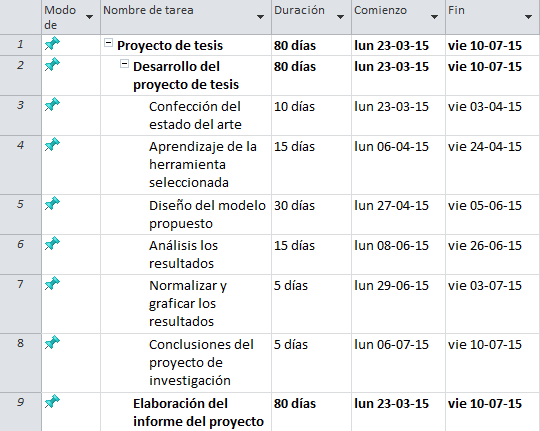
\includegraphics[scale=1]{images/CartaGantt.png}
\caption{Plan de trabajo}
\label{fig:cartagantt}
\end{figure}

\clearpage
\addcontentsline{toc}{section}{Referencias}
\bibliographystyle{unsrt}
\bibliography{references}

\end{document}